\documentclass[a4paper, 12pt]{article}
\usepackage{amsmath, amssymb, amsthm, stmaryrd}
\usepackage{geometry}
\usepackage{pgfplots}
\usepackage{tcolorbox}
\geometry{hmargin=2.5cm, vmargin=2.5cm}

\renewcommand*{\today}{28 novembre 2024}

\title{Analyse | CM: 11}
\author{Par Lorenzo}
\date{\today}

\newtheorem{theorem}{Théorème}[section]
\newtheorem{definition}{Définition}[section]
\newtheorem{example}{Example}[section]
\newtheorem{remark}{Remarques}[section]
\newtheorem{lemme}{Lemme}[section]
\newtheorem{corollaire}{Corollaire}[section]

\newtheorem{_proposition}{Proposition}[section]
\newenvironment{proposition}[1][]{
    \begin{_proposition}[#1]~\par
    \vspace*{0.5em}
}{%
    \end{_proposition}%
}

\newtheorem{_proprietes}{Propriétés}[section]
\newenvironment{proprietes}[1][]{
        \begin{_proprietes}[#1]~\par
        \vspace*{0.5em}
}{%
        \end{_proprietes}%
}

\newenvironment{rdem}[1][]{
    \begin{tcolorbox}[colframe=black, colback=white!10, sharp corners]
        #1
}{%
    \end{tcolorbox}
     
}

\newtheorem{_demonstration}{Démonstration}[section]
\newenvironment{demonstration}[1][]{
    \begin{_demonstration}[#1]~\par
    \vspace*{0.5em}
}{%
    \end{_demonstration}%
    \qed%
}

\newtheorem*{_demonstration*}{Démonstration}
\newenvironment{demonstration*}[1][]{
    \begin{_demonstration*}[#1]~\par
    \vspace*{0.5em}
}{%
    \end{_demonstration*}%
    \qed%
}

\newenvironment{ldefinition}{
    \begin{definition}~\par
    \vspace*{0.5em}
    \begin{enumerate}
}{
        \end{enumerate}
        \end{definition}
}

\newenvironment{lexample}{
    \begin{example}~\par
    \vspace*{0.5em}
    \begin{enumerate}
}{
        \end{enumerate}
        \end{example}
}

\newtheorem{_methode}{Méthode}[section]
\newenvironment{methode}{
    \begin{_methode}~\par
    \vspace*{0.5em}
}{
        \end{_methode}
}

\def\N{\mathbb{N}}
\def\Z{\mathbb{Z}}
\def\Q{\mathbb{Q}}
\def\R{\mathbb{R}}
\def\C{\mathbb{C}}
\def\K{\mathbb{K}}
\def\k{\Bbbk}

\def\un{(u_n)_{n \in \N}}
\def\xn#1{(#1_n)_{n \in \N}}

\def\o{\overline}
\def\eps{\varepsilon}

% \funcdef{name}{domain}{codomain}{variable}{expression}
% name: Name of the function (e.g. f)
% domain: Domain of the function (e.g. \mathbb{R})
% codomain: Codomain of the function (e.g. \mathbb{R})
% variable: Variables of the function (e.g. x)
% expression: Expression of the function (e.g. x^2)
\newcommand{\funcdef}[5]{%
    #1 :
    \begin{cases}
        #2 \rightarrow #3 \\
        #4 \mapsto #5
    \end{cases}
}

\newcommand{\lt}{\ensuremath <}
\newcommand{\gt}{\ensuremath >}

\begin{document}

\maketitle

\subsection{Fonctions inverses trigonométriques}

\begin{definition}
    La fonction cosinus $\cos: \begin{cases}\R \rightarrow [-1, 1]\\x \mapsto \cos(x)\end{cases}$

    Continue, périodique de période $2\pi$ et paire.
    
    \begin{tikzpicture}
        \begin{axis}[
            axis lines = middle,
            xlabel = $x$,
            ylabel = $y$,
            xmin = -2*pi, xmax = 2*pi,
            ymin = -1.5, ymax = 1.5,
            xtick = {-6.28318, -3.14159, 0, 3.14159, 6.28318},
            xticklabels = {$-2\pi$, $-\pi$, $0$, $\pi$, $2\pi$},
            ytick = {-1, 0, 1},
            grid = both,
            grid style = {line width=.1pt, draw=gray!10},
            major grid style = {line width=.2pt,draw=gray!50},
            width = 12cm,
            height = 8cm,
            ]
        \addplot[blue, domain=-2*pi:2*pi, samples=200] {cos(deg(x))};
        \end{axis}
    \end{tikzpicture}

    Sur l'intervalle $[0, \pi]$, la fonction $\cos$ est strictement décroissante et continue de $[0, \pi] \rightarrow [-1, 1]$
    D'apres le théorème de la bijection, il existe une fonction réciproque.
    
    Notée $\arccos: [-1, 1] \rightarrow [0, \pi]$ telle que
    
    $\cos(\arccos(x)) = x$, pour $x \in [-1, 1]$
    
    $\arccos(\cos(y)) = y$, pour $y \in [0, \pi]$

    \begin{tikzpicture}
        \begin{axis}[
            axis lines = middle,
            xlabel = $x$,
            ylabel = $y$,
            xmin = -1.5, xmax = 1.5,
            ymin = -0.5, ymax = 3.5,
            xtick = {-1, -0.5, 0, 0.5, 1},
            ytick = {0, 1.57079, 3.14159},
            yticklabels = {$0$, $\frac{\pi}{2}$, $\pi$},
            grid = both,
            grid style = {line width=.1pt, draw=gray!10},
            major grid style = {line width=.2pt,draw=gray!50},
            width = 12cm,
            height = 8cm,
        ]
        \addplot[red, domain=-1:1, samples=200] {rad(acos(x))};
        \end{axis}
    \end{tikzpicture}

\end{definition}

\begin{proprietes}
$\forall x \in ]-1, 1[, (\arccos(x))' = \dfrac{-1}{\sqrt{1-x^2}}$
\end{proprietes}

\begin{definition}
    La fonction sinus $\cos: \begin{cases}\R \rightarrow [-1, 1]\\x \mapsto \sin(x)\end{cases}$

    Continue, périodique de période $2\pi$ et paire.
    
    \begin{tikzpicture}
        \begin{axis}[
            axis lines = middle,
            xlabel = $x$,
            ylabel = $y$,
            xmin = -2*pi, xmax = 2*pi,
            ymin = -1.5, ymax = 1.5,
            xtick = {-6.28318, -3.14159, 0, 3.14159, 6.28318},
            xticklabels = {$-2\pi$, $-\pi$, $0$, $\pi$, $2\pi$},
            ytick = {-1, 0, 1},
            grid = both,
            grid style = {line width=.1pt, draw=gray!10},
            major grid style = {line width=.2pt,draw=gray!50},
            width = 12cm,
            height = 8cm,
            ]
        \addplot[blue, domain=-2*pi:2*pi, samples=200] {sin(deg(x))};
        \end{axis}
    \end{tikzpicture}

    Sur l'intervalle $[-\pi/2, \pi/2]$, la fonction $\sin$ est strictement décroissante et continue de $[-\pi/2, \pi/2] \rightarrow [-1, 1]$
    D'apres le théorème de la bijection, il existe une fonction réciproque.
    
    Notée $\arcsin: [-1, 1] \rightarrow [-\pi/2, \pi/2]$ telle que
    
    $\sin(\arcsin(x)) = x$, pour $x \in [-1, 1]$
    
    $\arcsin(\sin(y)) = y$, pour $y \in [-\pi/2, \pi/2]$

    \begin{tikzpicture}
        \begin{axis}[
            axis lines = middle,
            xlabel = $x$,
            ylabel = $y$,
            xmin = -1.5, xmax = 1.5,
            ymin = -2, ymax = 2,
            xtick = {-1, -0.5, 0, 0.5, 1},
            ytick = {-1.57079, 0, 1.57079},
            yticklabels = {$-\frac{\pi}{2}$, $0$, $\frac{\pi}{2}$},
            grid = both,
            grid style = {line width=.1pt, draw=gray!10},
            major grid style = {line width=.2pt,draw=gray!50},
            width = 12cm,
            height = 8cm,
        ]
        \addplot[red, domain=-1:1, samples=200] {rad(asin(x))};
        \end{axis}
    \end{tikzpicture}
\end{definition}

\begin{proprietes}
    $\forall x \in ]-1, 1[, (\arcsin(x))' = \dfrac{1}{\sqrt{1-x^2}}$
\end{proprietes}

\begin{definition}
    La fonction tangente $\tan(x) = \dfrac{\sin(x)}{\cos(x)}$ qui est défini sur
    $]\dfrac{-\pi}{2}, \dfrac{\pi}{2}[ \rightarrow \R$ est strictement croissante et continue.
    D'après le théorème de la bijection, il existe une fonction réciproque notée

    $\arctan: \R \rightarrow ]-\pi/2, \pi/2[$ l'angle de la tangente et vérifie
    
    $\tan(\arctan(x)) = x$ par $x \in \R$

    $\arctan(\tan(y)) = y$ pour $y \in ]-\pi/2, \pi/2[$

    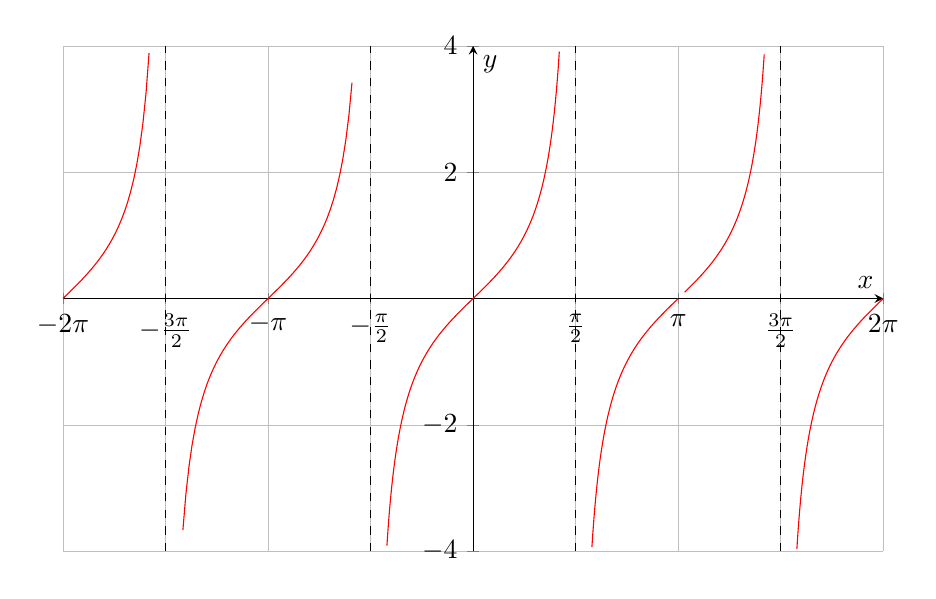
\begin{tikzpicture}
        \begin{axis}[
            axis lines = middle,
            xlabel = $x$,
            ylabel = $y$,
            xmin = -2*pi, xmax = 2*pi,
            ymin = -4, ymax = 4,
            xtick = {-6.28318, -4.71238, -3.14159, -1.5708, 0, 1.5708, 3.14159, 4.71238, 6.28318},
            xticklabels = {$-2\pi$, $-\frac{3\pi}{2}$, $-\pi$, $-\frac{\pi}{2}$, $0$, $\frac{\pi}{2}$, $\pi$, $\frac{3\pi}{2}$, $2\pi$},
            ytick = {-4, -2, 0, 2, 4},
            grid = both,
            grid style = {line width=.1pt, draw=gray!10},
            major grid style = {line width=.2pt,draw=gray!50},
            width = 12cm,
            height = 8cm,
            restrict y to domain=-4:4,
        ]
        \addplot[red, domain=-2*pi:-1.62, samples=100] {tan(deg(x))};
        \addplot[red, domain=-1.52:0, samples=100] {tan(deg(x))};
        \addplot[red, domain=0:1.52, samples=100] {tan(deg(x))};
        \addplot[red, domain=1.62:3.14, samples=100] {tan(deg(x))};
        \addplot[red, domain=3.24:4.66, samples=100] {tan(deg(x))};
        \addplot[red, domain=4.76:6.28, samples=100] {tan(deg(x))};
        
        % Asymptotes verticales
        \addplot[dashed] coordinates {(-4.71238, -4) (-4.71238, 4)};
        \addplot[dashed] coordinates {(-1.5708, -4) (-1.5708, 4)};
        \addplot[dashed] coordinates {(1.5708, -4) (1.5708, 4)};
        \addplot[dashed] coordinates {(4.71238, -4) (4.71238, 4)};
        \end{axis}
    \end{tikzpicture}

    \begin{tikzpicture}
        \begin{axis}[
            axis lines = middle,
            xlabel = $x$,
            ylabel = $y$,
            xmin = -10, xmax = 10,
            ymin = -2, ymax = 2,
            xtick = {-10, -5, 0, 5, 10},
            ytick = {-1.57079, 0, 1.57079},
            yticklabels = {$-\frac{\pi}{2}$, $0$, $\frac{\pi}{2}$},
            grid = both,
            grid style = {line width=.1pt, draw=gray!10},
            major grid style = {line width=.2pt,draw=gray!50},
            width = 12cm,
            height = 8cm,
        ]
        \addplot[blue, domain=-10:10, samples=200] {rad(atan(x))};
        
        % Asymptotes horizontales
        \addplot[dashed] coordinates {(-10, 1.57079) (10, 1.57079)};
        \addplot[dashed] coordinates {(-10, -1.57079) (10, -1.57079)};
        \end{axis}
    \end{tikzpicture}
\end{definition}

\begin{proprietes}
    $\forall x \in ]-1, 1[, (\arctan(x))' = \dfrac{1}{1+x^2}$
\end{proprietes}

\subsection{Fonctions hyperboliques inverses}

$e^ix = \cos(x) + i\sin(x) \iff \cos(x) = \dfrac{e^{ix} + e^{-ix}}{2} \iff \sin(x) = \dfrac{e^{ix} - e^{-ix}}{2}$

\begin{definition}
    On définit par $x \in \R$, le cosinus hyperbolique comme ($\cosh$ ou ch) \linebreak $\cosh(x) = \dfrac{e^x+e^{-x}}{2}$

    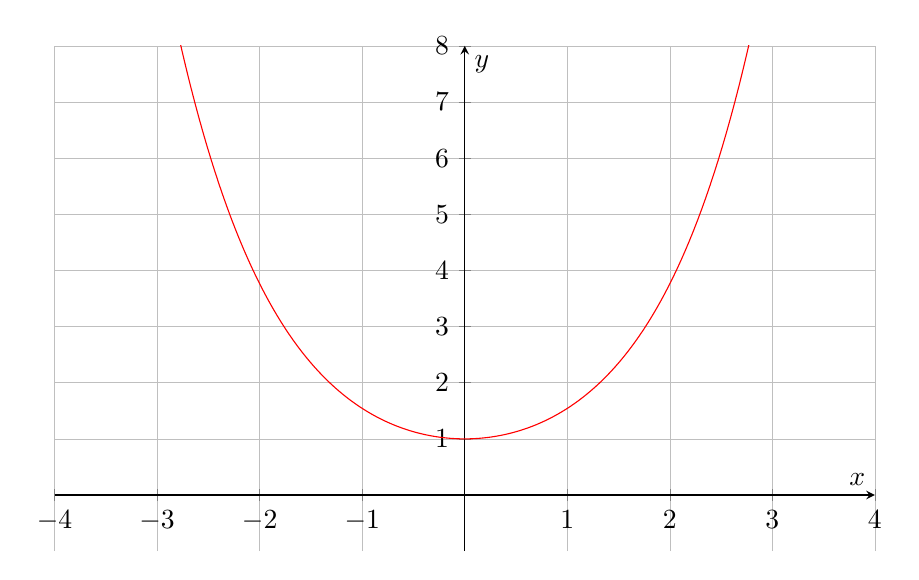
\begin{tikzpicture}
        \begin{axis}[
            axis lines = middle,
            xlabel = $x$,
            ylabel = $y$,
            xmin = -4, xmax = 4,
            ymin = -1, ymax = 8,
            xtick = {-4, -3, -2, -1, 0, 1, 2, 3, 4},
            ytick = {0, 1, 2, 3, 4, 5, 6, 7, 8},
            grid = both,
            grid style = {line width=.1pt, draw=gray!10},
            major grid style = {line width=.2pt,draw=gray!50},
            width = 12cm,
            height = 8cm,
        ]
        \addplot[red, domain=-4:4, samples=200] {(exp(x) + exp(-x))/2};
        \end{axis}
    \end{tikzpicture}

    La fonction $\cosh: [0, +\infty[ \rightarrow [1, +\infty[$ est strictement croissante et continue,
    elle définit une bijection et sa réciproque $\arg\cosh: [1, +\infty[ \rightarrow [0, +\infty[$

    $\arg\cosh(\cosh(x)) = x$ et $\cosh(\arg\cosh(x)) = x$

    \begin{tikzpicture}
        \begin{axis}[
            axis lines = middle,
            xlabel = $x$,
            ylabel = $y$,
            xmin = -1, xmax = 5,
            ymin = -0.5, ymax = 3,
            xtick = {1, 2, 3, 4, 5},
            ytick = {0, 1, 2, 3},
            grid = both,
            grid style = {line width=.1pt, draw=gray!10},
            major grid style = {line width=.2pt,draw=gray!50},
            width = 12cm,
            height = 8cm,
        ]
        \addplot[red, domain=1:5, samples=200] {ln(x + sqrt(x^2 - 1))};
        
        % Asymptote verticale
        \addplot[dashed] coordinates {(1, -0.5) (1, 3)};
        \end{axis}
    \end{tikzpicture}
\end{definition}

\begin{definition}
    On définit par $x \in \R$, le sinus hyperbolique comme ($\sinh$ ou sh) \linebreak $\cosh(x) = \dfrac{e^-+e^{-x}}{2}$

    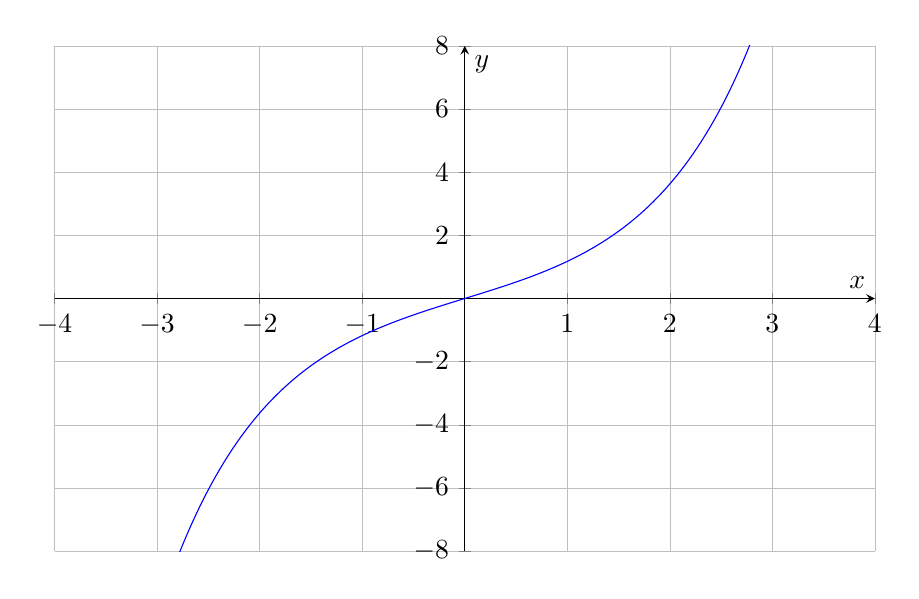
\begin{tikzpicture}
        \begin{axis}[
            axis lines = middle,
            xlabel = $x$,
            ylabel = $y$,
            xmin = -4, xmax = 4,
            ymin = -8, ymax = 8,
            xtick = {-4, -3, -2, -1, 0, 1, 2, 3, 4},
            ytick = {-8, -6, -4, -2, 0, 2, 4, 6, 8},
            grid = both,
            grid style = {line width=.1pt, draw=gray!10},
            major grid style = {line width=.2pt,draw=gray!50},
            width = 12cm,
            height = 8cm,
        ]
        \addplot[blue, domain=-4:4, samples=200] {(exp(x) - exp(-x))/2};
        \end{axis}
    \end{tikzpicture}

    La fonction $\sinh: \R \rightarrow \R$ est continue,
    elle définit une bijection et sa réciproque $\arg\sinh: \R \rightarrow \R$

    $\arg\sinh(\sinh(x)) = x$ et $\sinh(\arg\sinh(x)) = x$

    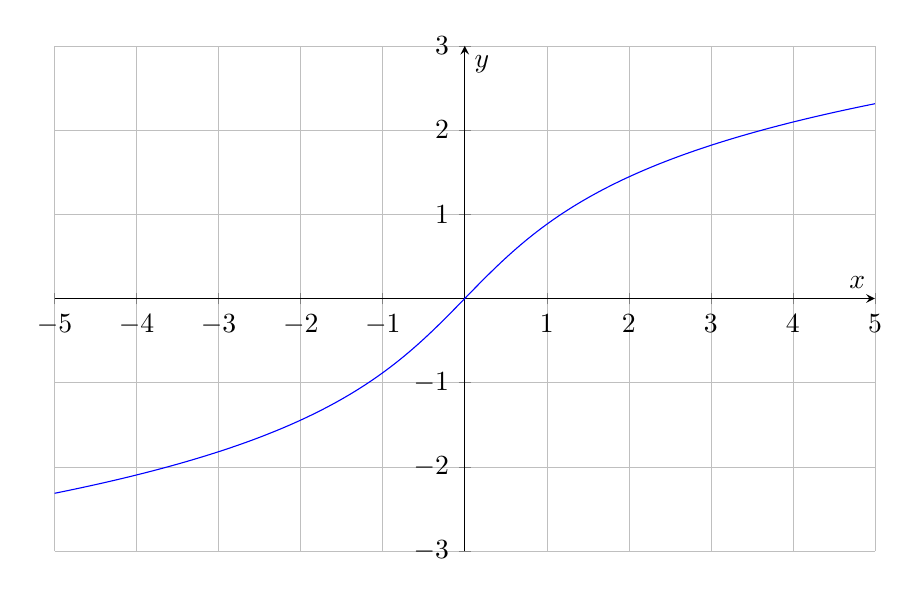
\begin{tikzpicture}
        \begin{axis}[
            axis lines = middle,
            xlabel = $x$,
            ylabel = $y$,
            xmin = -5, xmax = 5,
            ymin = -3, ymax = 3,
            xtick = {-5, -4, -3, -2, -1, 0, 1, 2, 3, 4, 5},
            ytick = {-3, -2, -1, 0, 1, 2, 3},
            grid = both,
            grid style = {line width=.1pt, draw=gray!10},
            major grid style = {line width=.2pt,draw=gray!50},
            width = 12cm,
            height = 8cm,
        ]
        \addplot[blue, domain=-5:5, samples=200] {ln(x + sqrt(1 + x^2))};
        \end{axis}
    \end{tikzpicture}
\end{definition}

\begin{definition}
    On définit par $x \in \R$, la tangente hyperbolique comme ($\tanh$ ou th) \linebreak $\tanh(x) = \dfrac{e^x-e^{-x}}{e^x+e^{-x}}$

    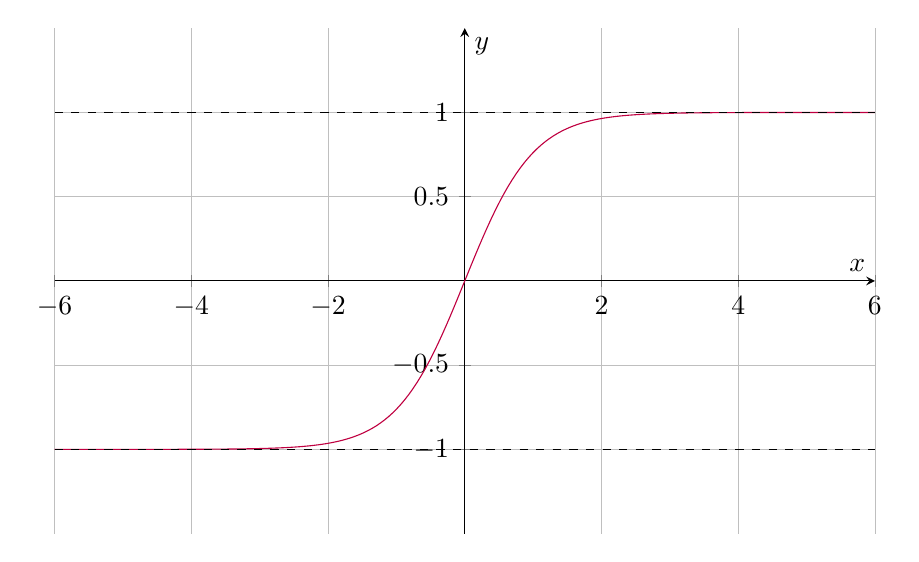
\begin{tikzpicture}
        \begin{axis}[
            axis lines = middle,
            xlabel = $x$,
            ylabel = $y$,
            xmin = -6, xmax = 6,
            ymin = -1.5, ymax = 1.5,
            xtick = {-6, -4, -2, 0, 2, 4, 6},
            ytick = {-1, -0.5, 0, 0.5, 1},
            grid = both,
            grid style = {line width=.1pt, draw=gray!10},
            major grid style = {line width=.2pt,draw=gray!50},
            width = 12cm,
            height = 8cm,
        ]
        \addplot[purple, domain=-6:6, samples=200] {(exp(x) - exp(-x))/(exp(x) + exp(-x))};
        
        % Asymptotes horizontales
        \addplot[dashed] coordinates {(-6, 1) (6, 1)};
        \addplot[dashed] coordinates {(-6, -1) (6, -1)};
        \end{axis}
        \end{tikzpicture}

    La fonction $\tanh: \R \rightarrow ]-1, 1[$ est continue,
    elle définit une bijection et sa réciproque $\arg\tanh: ]-1, 1[ \rightarrow \R$

    $\arg\tanh(\tanh(x)) = x$ et $\tanh(\arg\tanh(x)) = x$

    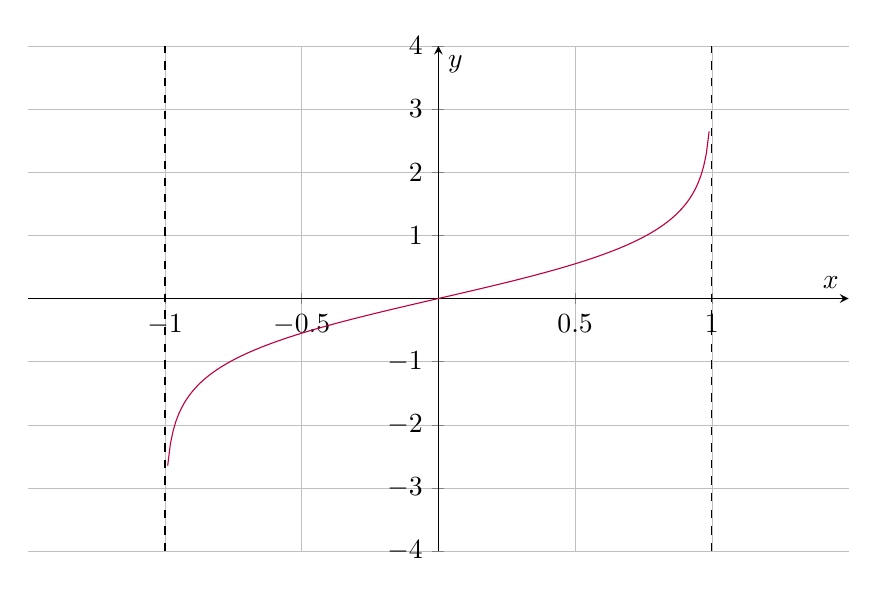
\begin{tikzpicture}
        \begin{axis}[
            axis lines = middle,
            xlabel = $x$,
            ylabel = $y$,
            xmin = -1.5, xmax = 1.5,
            ymin = -4, ymax = 4,
            xtick = {-1, -0.5, 0, 0.5, 1},
            ytick = {-4, -3, -2, -1, 0, 1, 2, 3, 4},
            grid = both,
            grid style = {line width=.1pt, draw=gray!10},
            major grid style = {line width=.2pt,draw=gray!50},
            width = 12cm,
            height = 8cm,
        ]
        \addplot[purple, domain=-0.99:0.99, samples=200] {0.5*ln((1+x)/(1-x))};
        
        % Asymptotes verticales
        \addplot[dashed] coordinates {(-1, -4) (-1, 4)};
        \addplot[dashed] coordinates {(1, -4) (1, 4)};
        \end{axis}
    \end{tikzpicture}
\end{definition}

\begin{proprietes}
    \begin{enumerate}
        \item $(\cosh(x))^2 - (\sinh(x)^2) = 1$
        \item \begin{itemize}
            \item $\cosh(a+b) = \cosh(a) \cosh(b) + \sinh(a) \sinh(b)$
            \item $\cosh(2a) = \cosh(a)^2 + \sinh(a)^2 = 2 \cosh(a)^2 - 1 = 1 + 2 \sinh(a)^2$
            \item $\sinh(a+b) = \sinh(a)\cosh(b) + \sinh(b)\cosh(a)$
            \item $\sinh(2a) = 2\sinh(a)\cosh(b)$
            \item $\tanh(a+b) = \dfrac{\tanh(a) \tanh(b)}{1 + \tanh(a) \tanh(b)}$
        \end{itemize}
        \item \begin{itemize}
            \item $(\cosh(x))' = \sinh(x)$
            \item $(\sinh(x))' = \cosh(x)$
            \item $(\tanh(x))' = 1 - \tanh(x)^2 = \dfrac{1}{\cosh(x)^2}$
        \end{itemize}
    \end{enumerate}
\end{proprietes}

\end{document}
